\section{Résolution d'un Snake Cube}
L'objectif visant à résoudre un Snake Cube est atteint. Notre application propose divers Snake Cube et les résout en un temps raisonnable (voir Chapitre~\ref{Tests}). En plus de résoudre des Snake Cube classiques, c'est-à-dire dont la forme finale est un cube, notre application propose des volume finaux plus complexes. Par exemple, on y trouve un Snake dont la forme finale s'apparente à un temple maya (\verb|snake_maya_temple.snake|).

\begin{figure}[h]
 \centering
 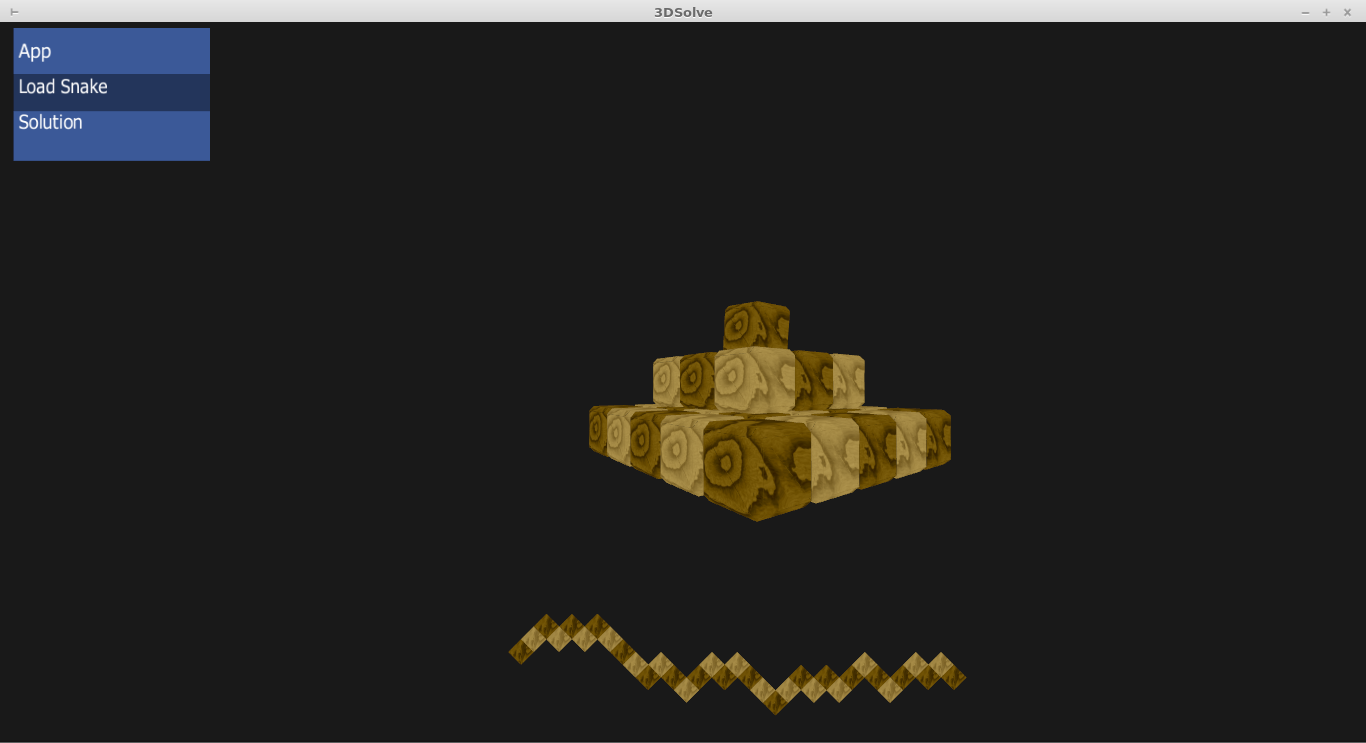
\includegraphics[scale=0.3,keepaspectratio=true]{img/screenShot3.png}
 \caption{``Temple maya'' résolu}
 \label{screenShot3}
\end{figure}

L'interface de rendu 3D permet à l'utilisateur de visualiser, à son rythme, diverses solutions menant à la résolution du casse-tête sélectionné.

\newpage
\section{Interactivité avec l'utilisateur}
L'objectif d'interactivité avec l'utilisateur, autrement dit la possibilité donnée à l'utilisateur de résoudre lui-même le casse-tête, est également atteint. En effet, notre application propose une interface 3D permettant à l'utilisateur de manipuler virtuellement le casse-tête et finalement, au prix d'un effort cérébral non négligeable, de le résoudre.

\begin{figure}[h]
 \centering
 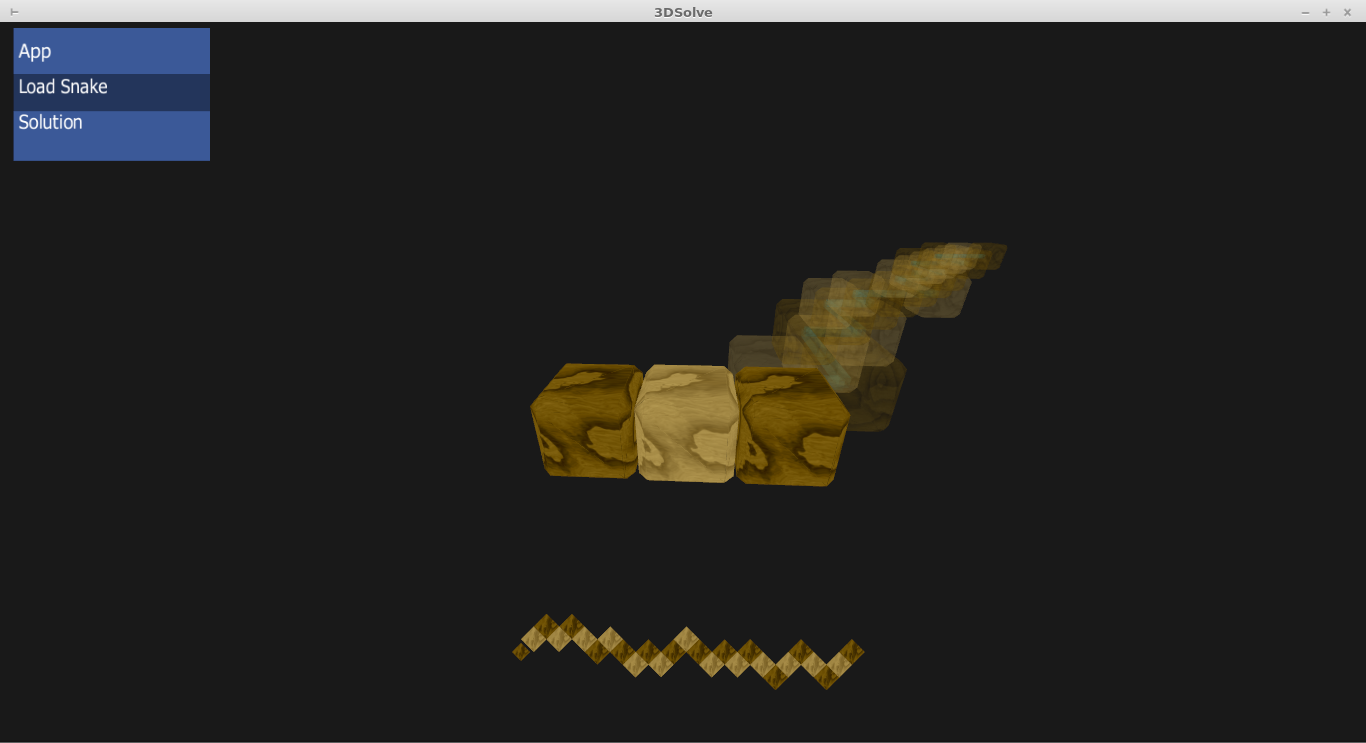
\includegraphics[scale=0.3,keepaspectratio=true]{img/screenShot1.png}
 \caption{Snake Cube déplié en attente de résolution}
 \label{screenShot1}
\end{figure}

\section{Amélioration proposée}
Nous avons eu diverses idées que nous aurions aimé implémenter si nous avions eu plus de temps. Nous les avons regroupées ici sous une seule et même proposition d'amélioration.

L'amélioration consiste en un éditeur de Snake Cube. Cet éditeur, sous la forme d'une interface dans le contexte de rendu 3D, permettrait à l'utilisateur de créer ses propres casse-tête.

En premier lieu, l'éditeur pourrait proposer à l'utilisateur de définir un volume en 3D puis de passer ce volume à un algorithme qui effectuerait le travail inverse de l'algorithme de résolution. C'est-à-dire qu'à partir du volume qui lui est donné, il recréerait l'agecement des unités du Snake correspondant. Le snake ainsi généré pourrait ensuite être sauvegardé dans le format défini au chapitre~\ref{ch6} afin d'être réutilisé, comme les autres Snakes, dans la partie interactive de l'application.

Ensuite, on pourrait également imaginer que cet éditeur permette à l'utilisateur de définir non seulement un volume mais également l'enchaînement des unités du snake afin de modéliser un snake réel qui n'est pas proposé par l'application.
